% Practice midterm: evaluating classifiers and SVMs.
% Build the test:      pdflatex practice_midterm.tex
% Build the solutions: pdflatex -jobname=practice_midterm_solutions "\def\withsolutions{}% Practice midterm: evaluating classifiers and SVMs.
% Build the test:      pdflatex practice_midterm.tex
% Build the solutions: pdflatex -jobname=practice_midterm_solutions "\def\withsolutions{}% Practice midterm: evaluating classifiers and SVMs.
% Build the test:      pdflatex practice_midterm.tex
% Build the solutions: pdflatex -jobname=practice_midterm_solutions "\def\withsolutions{}% Practice midterm: evaluating classifiers and SVMs.
% Build the test:      pdflatex practice_midterm.tex
% Build the solutions: pdflatex -jobname=practice_midterm_solutions "\def\withsolutions{}\input{practice_midterm}"
\documentclass[11pt,addpoints]{exam}
\ifdefined\withsolutions \printanswers \fi
\usepackage[margin=1in]{geometry}
\usepackage{amsmath,amssymb,bm,booktabs,tikz}
\usepackage[T1]{fontenc}
\usepackage{lmodern}

% parts numbered 1.1, 1.2, ...; subparts (a), (b), ...
\renewcommand{\thepartno}{\thequestion.\arabic{partno}}
\renewcommand{\partlabel}{\thepartno}
\renewcommand{\thesubpart}{\alph{subpart}}
\renewcommand{\subpartlabel}{(\thesubpart)}
\qformat{\large\bfseries \thequestion.\ \thequestiontitle\hfill}
\pointname{ points}
\pointformat{(\thepoints)}
\bracketedpoints
\unframedsolutions
\renewcommand{\solutiontitle}{\noindent\textbf{Solution:}\enspace}

% an empty ROC plot (unit square, ticks every 0.2) for students to draw in
\newcommand{\rocaxes}{%
  \draw[step=0.2,gray!30,very thin] (0,0) grid (1,1);
  \draw[->] (0,0) -- (1.08,0) node[right] {FPR};
  \draw[->] (0,0) -- (0,1.08) node[above] {TPR};
  \foreach \t in {0,0.2,0.4,0.6,0.8,1} {
    \draw (\t,0) -- (\t,-0.02) node[below] {\small\t};
    \draw (0,\t) -- (-0.02,\t) node[left] {\small\t};}}

\begin{document}
\begin{center}
  {\Large\bfseries Machine Learning: Practice Midterm}\\[4pt]
  \ifprintanswers Solutions \else Name: \rule{6cm}{0.4pt} \fi
\end{center}
\vspace{1em}

\begin{questions}

% ===================================================================== 1
\titledquestion{Evaluating classifiers (20 points)}
A charity trains African giant pouched rats (``HeroRATs'') to detect tuberculosis (TB) via their
impressive sense of smell. To make sure the rats are effective, each rat is tested on 1000 samples
of sputum. Suppose a laboratory test shows that 100 of them come from patients with TB. The rat
pauses at 80\% of the TB samples and at 10\% of the others. Treat ``has TB'' as the positive class.

\begin{parts}
\part[4] Write down the confusion matrix.
\begin{solution}
100 TB samples and 900 non-TB samples. $\mathrm{TP} = 0.8 \times 100$, $\mathrm{FP} = 0.1 \times 900$.
\begin{center}
\begin{tabular}{lcc}
\toprule
 & rat pauses & rat moves on \\
\midrule
TB    & TP $= 80$ & FN $= 20$ \\
no TB & FP $= 90$ & TN $= 810$ \\
\bottomrule
\end{tabular}
\end{center}
\end{solution}

\part[2] What are precision and recall for this rat?
\begin{solution}
Precision $= 80/(80+90) = 80/170 \approx 0.47$. \quad Recall $= 80/100 = 0.80$.
\end{solution}

\part[2] Do we care more about improving precision or recall for this problem, and why?
\begin{solution}
Recall. A missed TB patient (false negative) goes untreated and keeps infecting others; a false
alarm (false positive) only costs one extra laboratory test.
\end{solution}

\uplevel{The rat handler also records how long the rat pauses at each sample before moving on. Here are 10
samples, 5 from TB patients and 5 without TB:
\begin{center}
\begin{tabular}{lcccccccccc}
\toprule
sample          & A & B & C & D & E & F & G & H & I & J \\
\midrule
pause (seconds) & 2.6 & 0.6 & 4.6 & 2.0 & 1.3 & 3.7 & 4.2 & 1.0 & 3.0 & 2.4 \\
TB?             & yes & no & yes & no & yes & no & yes & no & yes & no \\
\bottomrule
\end{tabular}
\end{center}
We say a rat flags a sample as TB if it pauses for over $t$ seconds.}

\part[10] Draw the ROC curve.
\ifprintanswers\else
\begin{center}
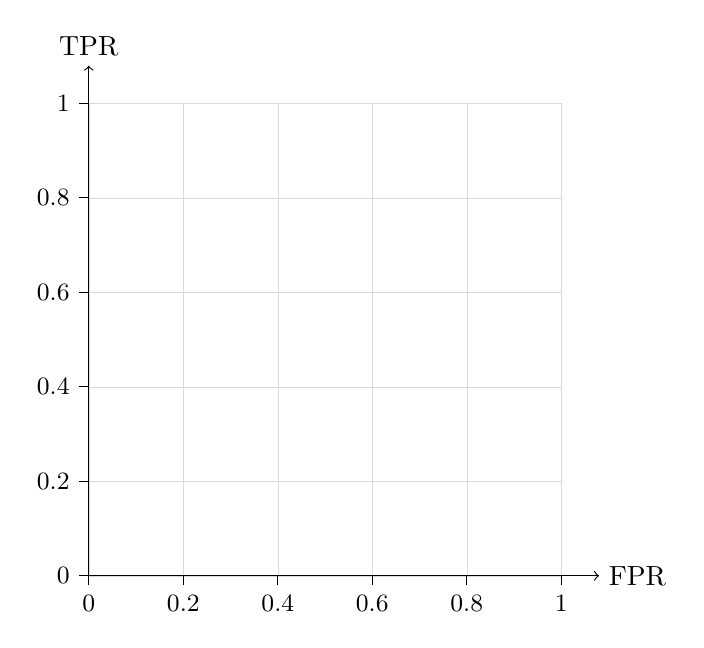
\begin{tikzpicture}[scale=6]\rocaxes\end{tikzpicture}
\end{center}
\fi
\begin{solution}
Sorted by pause, longest first: C (TB), G (TB), F (no), I (TB), A (TB), J (no), D (no), E (TB),
H (no), B (no). As $t$ passes each sample, a TB sample moves the point up by $1/5 = 0.2$ and a
non-TB sample moves it right by $0.2$. Starting at $(0,0)$, the points are
\[
(0,0.2),\ (0,0.4),\ (0.2,0.4),\ (0.2,0.6),\ (0.2,0.8),\ (0.4,0.8),\ (0.6,0.8),\ (0.6,1),\ (0.8,1),\ (1,1).
\]
\begin{center}
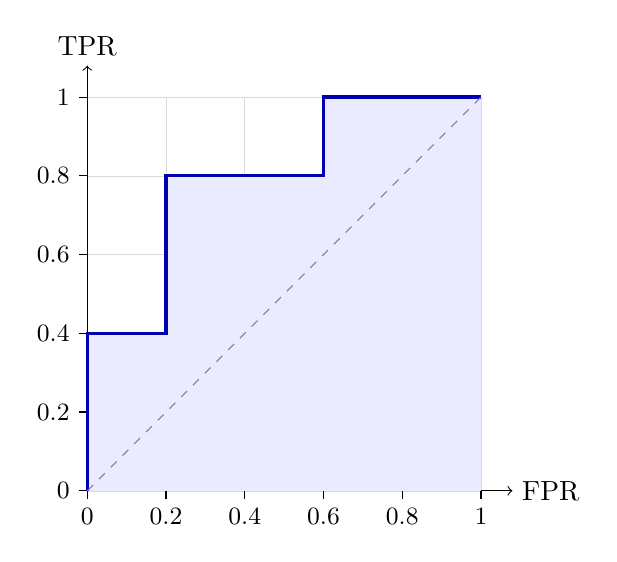
\begin{tikzpicture}[scale=5]
\rocaxes
\fill[blue!8] (0,0) -- (0,0.4) -- (0.2,0.4) -- (0.2,0.8) -- (0.6,0.8) -- (0.6,1) -- (1,1) -- (1,0) -- cycle;
\draw[very thick,blue!70!black] (0,0) -- (0,0.4) -- (0.2,0.4) -- (0.2,0.8) -- (0.6,0.8) -- (0.6,1) -- (1,1);
\draw[dashed,gray] (0,0) -- (1,1);
\end{tikzpicture}
\end{center}
\end{solution}

\part[2] Compute the AUC.
\begin{solution}
The area under the staircase, in columns of width $0.2$ with heights $0.4, 0.8, 0.8, 1, 1$:
$\mathrm{AUC} = 0.2 \times (0.4 + 0.8 + 0.8 + 1 + 1) = 0.80$.
\end{solution}
\end{parts}

% ===================================================================== 2
\titledquestion{Support vector machines (20 points)}
\begin{parts}
\part[10] A soft-margin SVM returned $\bm{w} = (4, 3)$, $b = -12$.
\begin{center}
\begin{tabular}{lccccc}
\toprule
point  & A & B & C & D & E \\
\midrule
$x_1$  & 3 & 1 & 2.5 & 1 & 3 \\
$x_2$  & 1 & 2 & 1 & 2.5 & 0.5 \\
label  & $+$ & $-$ & $+$ & $-$ & $-$ \\
\bottomrule
\end{tabular}
\end{center}
\begin{subparts}
\subpart Compute $f(\bm{x})$ and the predicted class of each point.
\subpart What is the width of the margin?
\subpart Compute each point's distance to the decision boundary.
\subpart Which points are support vectors? Which point is on the margin, which is inside it, and
which is misclassified?
\end{subparts}
\begin{solution}
$f(\bm{x}) = 4x_1 + 3x_2 - 12$ and $\|\bm{w}\| = \sqrt{4^2 + 3^2} = 5$.
\begin{center}
\begin{tabular}{lccccc}
\toprule
point & A & B & C & D & E \\
\midrule
$f(\bm{x})$                     & $3$   & $-2$  & $1$   & $-0.5$ & $1.5$ \\
predicted class                 & $+$   & $-$   & $+$   & $-$    & $+$ \\
distance $|f(\bm{x})|/\|\bm{w}\|$ & $0.6$ & $0.4$ & $0.2$ & $0.1$  & $0.3$ \\
$y\,f(\bm{x})$                  & $3$   & $2$   & $1$   & $0.5$  & $-1.5$ \\
\bottomrule
\end{tabular}
\end{center}
(b) Margin width $= 2/\|\bm{w}\| = 2/5 = 0.4$.

(d) The support vectors are the points with $y\,f(\bm{x}) \le 1$: C, D and E. C is on the margin
($y\,f = 1$), D is inside the margin but correctly classified ($y\,f = 0.5$), and E is
misclassified (label $-$, predicted $+$).
\end{solution}

\part[6] Write down the objective function for the soft-margin SVM and explain why this is what we
want to optimize.
\begin{solution}
\[
\min_{\bm{w},\, b,\, \bm{\xi}} \ \tfrac12 \|\bm{w}\|^2 + C \sum_i \xi_i
\quad \text{subject to} \quad y_i(\bm{w} \cdot \bm{x}_i + b) \ge 1 - \xi_i,\ \ \xi_i \ge 0 .
\]
Minimizing $\tfrac12\|\bm{w}\|^2$ maximizes the margin $2/\|\bm{w}\|$. The slack $\xi_i$ measures
how far point $i$ falls short of being on the correct side, outside the margin; the sum penalizes
these violations. $C$ sets the trade-off between a wide margin and few violations.
\end{solution}

\part[2] Suppose our soft-margin SVM obtains 95\% training accuracy but 60\% validation accuracy.
What does this suggest about our hyperparameter $C$?
\begin{solution}
The large gap between training and validation accuracy means the model overfits. $C$ is probably
too large: violations are so expensive that the margin narrows to fit individual training points.
Try a smaller $C$ (wider margin, more slack), chosen on validation data.
\end{solution}

\part[2] What are support vectors? Is every training datapoint that falls inside the margin a
support vector?
\begin{solution}
Support vectors are the training points that determine the solution: the points on the margin,
inside it, or misclassified, that is, those with $y_i f(\bm{x}_i) \le 1$. Moving any other point
(while it stays outside the margin) does not change the SVM. Yes: every point inside the margin is a
support vector.
\end{solution}
\end{parts}

\end{questions}
\end{document}
"
\documentclass[11pt,addpoints]{exam}
\ifdefined\withsolutions \printanswers \fi
\usepackage[margin=1in]{geometry}
\usepackage{amsmath,amssymb,bm,booktabs,tikz}
\usepackage[T1]{fontenc}
\usepackage{lmodern}

% parts numbered 1.1, 1.2, ...; subparts (a), (b), ...
\renewcommand{\thepartno}{\thequestion.\arabic{partno}}
\renewcommand{\partlabel}{\thepartno}
\renewcommand{\thesubpart}{\alph{subpart}}
\renewcommand{\subpartlabel}{(\thesubpart)}
\qformat{\large\bfseries \thequestion.\ \thequestiontitle\hfill}
\pointname{ points}
\pointformat{(\thepoints)}
\bracketedpoints
\unframedsolutions
\renewcommand{\solutiontitle}{\noindent\textbf{Solution:}\enspace}

% an empty ROC plot (unit square, ticks every 0.2) for students to draw in
\newcommand{\rocaxes}{%
  \draw[step=0.2,gray!30,very thin] (0,0) grid (1,1);
  \draw[->] (0,0) -- (1.08,0) node[right] {FPR};
  \draw[->] (0,0) -- (0,1.08) node[above] {TPR};
  \foreach \t in {0,0.2,0.4,0.6,0.8,1} {
    \draw (\t,0) -- (\t,-0.02) node[below] {\small\t};
    \draw (0,\t) -- (-0.02,\t) node[left] {\small\t};}}

\begin{document}
\begin{center}
  {\Large\bfseries Machine Learning: Practice Midterm}\\[4pt]
  \ifprintanswers Solutions \else Name: \rule{6cm}{0.4pt} \fi
\end{center}
\vspace{1em}

\begin{questions}

% ===================================================================== 1
\titledquestion{Evaluating classifiers (20 points)}
A charity trains African giant pouched rats (``HeroRATs'') to detect tuberculosis (TB) via their
impressive sense of smell. To make sure the rats are effective, each rat is tested on 1000 samples
of sputum. Suppose a laboratory test shows that 100 of them come from patients with TB. The rat
pauses at 80\% of the TB samples and at 10\% of the others. Treat ``has TB'' as the positive class.

\begin{parts}
\part[4] Write down the confusion matrix.
\begin{solution}
100 TB samples and 900 non-TB samples. $\mathrm{TP} = 0.8 \times 100$, $\mathrm{FP} = 0.1 \times 900$.
\begin{center}
\begin{tabular}{lcc}
\toprule
 & rat pauses & rat moves on \\
\midrule
TB    & TP $= 80$ & FN $= 20$ \\
no TB & FP $= 90$ & TN $= 810$ \\
\bottomrule
\end{tabular}
\end{center}
\end{solution}

\part[2] What are precision and recall for this rat?
\begin{solution}
Precision $= 80/(80+90) = 80/170 \approx 0.47$. \quad Recall $= 80/100 = 0.80$.
\end{solution}

\part[2] Do we care more about improving precision or recall for this problem, and why?
\begin{solution}
Recall. A missed TB patient (false negative) goes untreated and keeps infecting others; a false
alarm (false positive) only costs one extra laboratory test.
\end{solution}

\uplevel{The rat handler also records how long the rat pauses at each sample before moving on. Here are 10
samples, 5 from TB patients and 5 without TB:
\begin{center}
\begin{tabular}{lcccccccccc}
\toprule
sample          & A & B & C & D & E & F & G & H & I & J \\
\midrule
pause (seconds) & 2.6 & 0.6 & 4.6 & 2.0 & 1.3 & 3.7 & 4.2 & 1.0 & 3.0 & 2.4 \\
TB?             & yes & no & yes & no & yes & no & yes & no & yes & no \\
\bottomrule
\end{tabular}
\end{center}
We say a rat flags a sample as TB if it pauses for over $t$ seconds.}

\part[10] Draw the ROC curve.
\ifprintanswers\else
\begin{center}
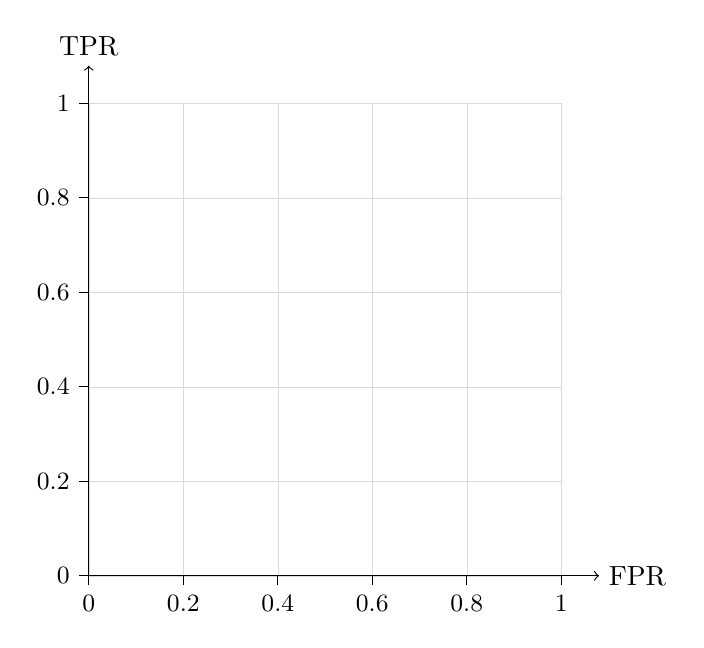
\begin{tikzpicture}[scale=6]\rocaxes\end{tikzpicture}
\end{center}
\fi
\begin{solution}
Sorted by pause, longest first: C (TB), G (TB), F (no), I (TB), A (TB), J (no), D (no), E (TB),
H (no), B (no). As $t$ passes each sample, a TB sample moves the point up by $1/5 = 0.2$ and a
non-TB sample moves it right by $0.2$. Starting at $(0,0)$, the points are
\[
(0,0.2),\ (0,0.4),\ (0.2,0.4),\ (0.2,0.6),\ (0.2,0.8),\ (0.4,0.8),\ (0.6,0.8),\ (0.6,1),\ (0.8,1),\ (1,1).
\]
\begin{center}
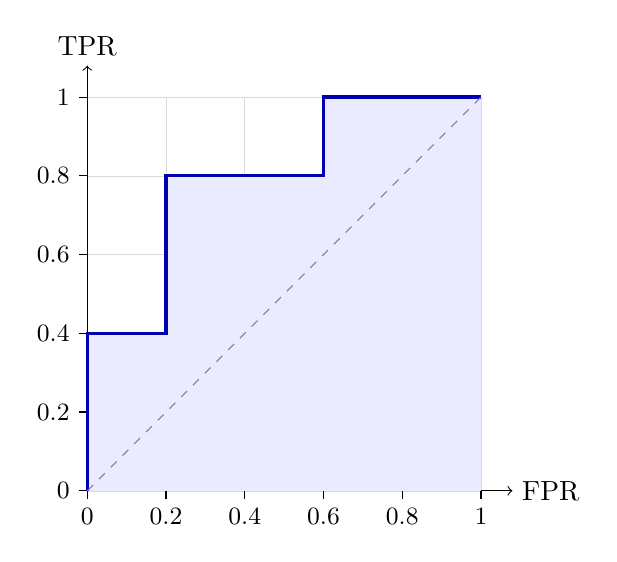
\begin{tikzpicture}[scale=5]
\rocaxes
\fill[blue!8] (0,0) -- (0,0.4) -- (0.2,0.4) -- (0.2,0.8) -- (0.6,0.8) -- (0.6,1) -- (1,1) -- (1,0) -- cycle;
\draw[very thick,blue!70!black] (0,0) -- (0,0.4) -- (0.2,0.4) -- (0.2,0.8) -- (0.6,0.8) -- (0.6,1) -- (1,1);
\draw[dashed,gray] (0,0) -- (1,1);
\end{tikzpicture}
\end{center}
\end{solution}

\part[2] Compute the AUC.
\begin{solution}
The area under the staircase, in columns of width $0.2$ with heights $0.4, 0.8, 0.8, 1, 1$:
$\mathrm{AUC} = 0.2 \times (0.4 + 0.8 + 0.8 + 1 + 1) = 0.80$.
\end{solution}
\end{parts}

% ===================================================================== 2
\titledquestion{Support vector machines (20 points)}
\begin{parts}
\part[10] A soft-margin SVM returned $\bm{w} = (4, 3)$, $b = -12$.
\begin{center}
\begin{tabular}{lccccc}
\toprule
point  & A & B & C & D & E \\
\midrule
$x_1$  & 3 & 1 & 2.5 & 1 & 3 \\
$x_2$  & 1 & 2 & 1 & 2.5 & 0.5 \\
label  & $+$ & $-$ & $+$ & $-$ & $-$ \\
\bottomrule
\end{tabular}
\end{center}
\begin{subparts}
\subpart Compute $f(\bm{x})$ and the predicted class of each point.
\subpart What is the width of the margin?
\subpart Compute each point's distance to the decision boundary.
\subpart Which points are support vectors? Which point is on the margin, which is inside it, and
which is misclassified?
\end{subparts}
\begin{solution}
$f(\bm{x}) = 4x_1 + 3x_2 - 12$ and $\|\bm{w}\| = \sqrt{4^2 + 3^2} = 5$.
\begin{center}
\begin{tabular}{lccccc}
\toprule
point & A & B & C & D & E \\
\midrule
$f(\bm{x})$                     & $3$   & $-2$  & $1$   & $-0.5$ & $1.5$ \\
predicted class                 & $+$   & $-$   & $+$   & $-$    & $+$ \\
distance $|f(\bm{x})|/\|\bm{w}\|$ & $0.6$ & $0.4$ & $0.2$ & $0.1$  & $0.3$ \\
$y\,f(\bm{x})$                  & $3$   & $2$   & $1$   & $0.5$  & $-1.5$ \\
\bottomrule
\end{tabular}
\end{center}
(b) Margin width $= 2/\|\bm{w}\| = 2/5 = 0.4$.

(d) The support vectors are the points with $y\,f(\bm{x}) \le 1$: C, D and E. C is on the margin
($y\,f = 1$), D is inside the margin but correctly classified ($y\,f = 0.5$), and E is
misclassified (label $-$, predicted $+$).
\end{solution}

\part[6] Write down the objective function for the soft-margin SVM and explain why this is what we
want to optimize.
\begin{solution}
\[
\min_{\bm{w},\, b,\, \bm{\xi}} \ \tfrac12 \|\bm{w}\|^2 + C \sum_i \xi_i
\quad \text{subject to} \quad y_i(\bm{w} \cdot \bm{x}_i + b) \ge 1 - \xi_i,\ \ \xi_i \ge 0 .
\]
Minimizing $\tfrac12\|\bm{w}\|^2$ maximizes the margin $2/\|\bm{w}\|$. The slack $\xi_i$ measures
how far point $i$ falls short of being on the correct side, outside the margin; the sum penalizes
these violations. $C$ sets the trade-off between a wide margin and few violations.
\end{solution}

\part[2] Suppose our soft-margin SVM obtains 95\% training accuracy but 60\% validation accuracy.
What does this suggest about our hyperparameter $C$?
\begin{solution}
The large gap between training and validation accuracy means the model overfits. $C$ is probably
too large: violations are so expensive that the margin narrows to fit individual training points.
Try a smaller $C$ (wider margin, more slack), chosen on validation data.
\end{solution}

\part[2] What are support vectors? Is every training datapoint that falls inside the margin a
support vector?
\begin{solution}
Support vectors are the training points that determine the solution: the points on the margin,
inside it, or misclassified, that is, those with $y_i f(\bm{x}_i) \le 1$. Moving any other point
(while it stays outside the margin) does not change the SVM. Yes: every point inside the margin is a
support vector.
\end{solution}
\end{parts}

\end{questions}
\end{document}
"
\documentclass[11pt,addpoints]{exam}
\ifdefined\withsolutions \printanswers \fi
\usepackage[margin=1in]{geometry}
\usepackage{amsmath,amssymb,bm,booktabs,tikz}
\usepackage[T1]{fontenc}
\usepackage{lmodern}

% parts numbered 1.1, 1.2, ...; subparts (a), (b), ...
\renewcommand{\thepartno}{\thequestion.\arabic{partno}}
\renewcommand{\partlabel}{\thepartno}
\renewcommand{\thesubpart}{\alph{subpart}}
\renewcommand{\subpartlabel}{(\thesubpart)}
\qformat{\large\bfseries \thequestion.\ \thequestiontitle\hfill}
\pointname{ points}
\pointformat{(\thepoints)}
\bracketedpoints
\unframedsolutions
\renewcommand{\solutiontitle}{\noindent\textbf{Solution:}\enspace}

% an empty ROC plot (unit square, ticks every 0.2) for students to draw in
\newcommand{\rocaxes}{%
  \draw[step=0.2,gray!30,very thin] (0,0) grid (1,1);
  \draw[->] (0,0) -- (1.08,0) node[right] {FPR};
  \draw[->] (0,0) -- (0,1.08) node[above] {TPR};
  \foreach \t in {0,0.2,0.4,0.6,0.8,1} {
    \draw (\t,0) -- (\t,-0.02) node[below] {\small\t};
    \draw (0,\t) -- (-0.02,\t) node[left] {\small\t};}}

\begin{document}
\begin{center}
  {\Large\bfseries Machine Learning: Practice Midterm}\\[4pt]
  \ifprintanswers Solutions \else Name: \rule{6cm}{0.4pt} \fi
\end{center}
\vspace{1em}

\begin{questions}

% ===================================================================== 1
\titledquestion{Evaluating classifiers (20 points)}
A charity trains African giant pouched rats (``HeroRATs'') to detect tuberculosis (TB) via their
impressive sense of smell. To make sure the rats are effective, each rat is tested on 1000 samples
of sputum. Suppose a laboratory test shows that 100 of them come from patients with TB. The rat
pauses at 80\% of the TB samples and at 10\% of the others. Treat ``has TB'' as the positive class.

\begin{parts}
\part[4] Write down the confusion matrix.
\begin{solution}
100 TB samples and 900 non-TB samples. $\mathrm{TP} = 0.8 \times 100$, $\mathrm{FP} = 0.1 \times 900$.
\begin{center}
\begin{tabular}{lcc}
\toprule
 & rat pauses & rat moves on \\
\midrule
TB    & TP $= 80$ & FN $= 20$ \\
no TB & FP $= 90$ & TN $= 810$ \\
\bottomrule
\end{tabular}
\end{center}
\end{solution}

\part[2] What are precision and recall for this rat?
\begin{solution}
Precision $= 80/(80+90) = 80/170 \approx 0.47$. \quad Recall $= 80/100 = 0.80$.
\end{solution}

\part[2] Do we care more about improving precision or recall for this problem, and why?
\begin{solution}
Recall. A missed TB patient (false negative) goes untreated and keeps infecting others; a false
alarm (false positive) only costs one extra laboratory test.
\end{solution}

\uplevel{The rat handler also records how long the rat pauses at each sample before moving on. Here are 10
samples, 5 from TB patients and 5 without TB:
\begin{center}
\begin{tabular}{lcccccccccc}
\toprule
sample          & A & B & C & D & E & F & G & H & I & J \\
\midrule
pause (seconds) & 2.6 & 0.6 & 4.6 & 2.0 & 1.3 & 3.7 & 4.2 & 1.0 & 3.0 & 2.4 \\
TB?             & yes & no & yes & no & yes & no & yes & no & yes & no \\
\bottomrule
\end{tabular}
\end{center}
We say a rat flags a sample as TB if it pauses for over $t$ seconds.}

\part[10] Draw the ROC curve.
\ifprintanswers\else
\begin{center}
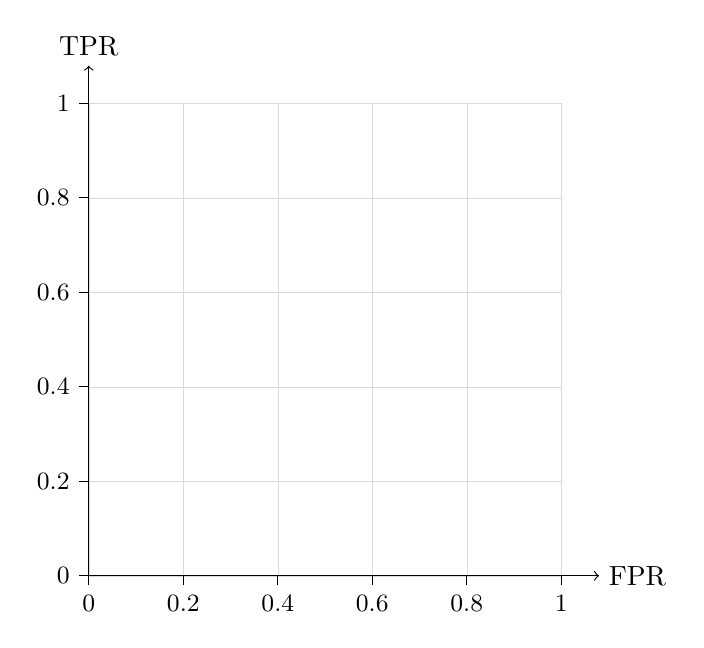
\begin{tikzpicture}[scale=6]\rocaxes\end{tikzpicture}
\end{center}
\fi
\begin{solution}
Sorted by pause, longest first: C (TB), G (TB), F (no), I (TB), A (TB), J (no), D (no), E (TB),
H (no), B (no). As $t$ passes each sample, a TB sample moves the point up by $1/5 = 0.2$ and a
non-TB sample moves it right by $0.2$. Starting at $(0,0)$, the points are
\[
(0,0.2),\ (0,0.4),\ (0.2,0.4),\ (0.2,0.6),\ (0.2,0.8),\ (0.4,0.8),\ (0.6,0.8),\ (0.6,1),\ (0.8,1),\ (1,1).
\]
\begin{center}
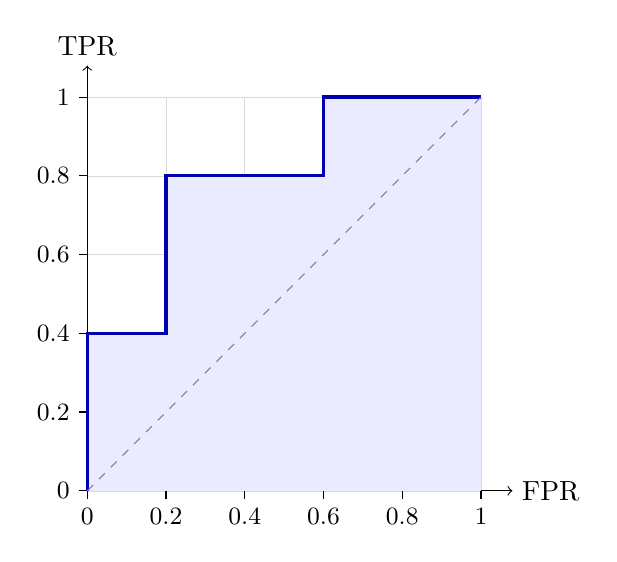
\begin{tikzpicture}[scale=5]
\rocaxes
\fill[blue!8] (0,0) -- (0,0.4) -- (0.2,0.4) -- (0.2,0.8) -- (0.6,0.8) -- (0.6,1) -- (1,1) -- (1,0) -- cycle;
\draw[very thick,blue!70!black] (0,0) -- (0,0.4) -- (0.2,0.4) -- (0.2,0.8) -- (0.6,0.8) -- (0.6,1) -- (1,1);
\draw[dashed,gray] (0,0) -- (1,1);
\end{tikzpicture}
\end{center}
\end{solution}

\part[2] Compute the AUC.
\begin{solution}
The area under the staircase, in columns of width $0.2$ with heights $0.4, 0.8, 0.8, 1, 1$:
$\mathrm{AUC} = 0.2 \times (0.4 + 0.8 + 0.8 + 1 + 1) = 0.80$.
\end{solution}
\end{parts}

% ===================================================================== 2
\titledquestion{Support vector machines (20 points)}
\begin{parts}
\part[10] A soft-margin SVM returned $\bm{w} = (4, 3)$, $b = -12$.
\begin{center}
\begin{tabular}{lccccc}
\toprule
point  & A & B & C & D & E \\
\midrule
$x_1$  & 3 & 1 & 2.5 & 1 & 3 \\
$x_2$  & 1 & 2 & 1 & 2.5 & 0.5 \\
label  & $+$ & $-$ & $+$ & $-$ & $-$ \\
\bottomrule
\end{tabular}
\end{center}
\begin{subparts}
\subpart Compute $f(\bm{x})$ and the predicted class of each point.
\subpart What is the width of the margin?
\subpart Compute each point's distance to the decision boundary.
\subpart Which points are support vectors? Which point is on the margin, which is inside it, and
which is misclassified?
\end{subparts}
\begin{solution}
$f(\bm{x}) = 4x_1 + 3x_2 - 12$ and $\|\bm{w}\| = \sqrt{4^2 + 3^2} = 5$.
\begin{center}
\begin{tabular}{lccccc}
\toprule
point & A & B & C & D & E \\
\midrule
$f(\bm{x})$                     & $3$   & $-2$  & $1$   & $-0.5$ & $1.5$ \\
predicted class                 & $+$   & $-$   & $+$   & $-$    & $+$ \\
distance $|f(\bm{x})|/\|\bm{w}\|$ & $0.6$ & $0.4$ & $0.2$ & $0.1$  & $0.3$ \\
$y\,f(\bm{x})$                  & $3$   & $2$   & $1$   & $0.5$  & $-1.5$ \\
\bottomrule
\end{tabular}
\end{center}
(b) Margin width $= 2/\|\bm{w}\| = 2/5 = 0.4$.

(d) The support vectors are the points with $y\,f(\bm{x}) \le 1$: C, D and E. C is on the margin
($y\,f = 1$), D is inside the margin but correctly classified ($y\,f = 0.5$), and E is
misclassified (label $-$, predicted $+$).
\end{solution}

\part[6] Write down the objective function for the soft-margin SVM and explain why this is what we
want to optimize.
\begin{solution}
\[
\min_{\bm{w},\, b,\, \bm{\xi}} \ \tfrac12 \|\bm{w}\|^2 + C \sum_i \xi_i
\quad \text{subject to} \quad y_i(\bm{w} \cdot \bm{x}_i + b) \ge 1 - \xi_i,\ \ \xi_i \ge 0 .
\]
Minimizing $\tfrac12\|\bm{w}\|^2$ maximizes the margin $2/\|\bm{w}\|$. The slack $\xi_i$ measures
how far point $i$ falls short of being on the correct side, outside the margin; the sum penalizes
these violations. $C$ sets the trade-off between a wide margin and few violations.
\end{solution}

\part[2] Suppose our soft-margin SVM obtains 95\% training accuracy but 60\% validation accuracy.
What does this suggest about our hyperparameter $C$?
\begin{solution}
The large gap between training and validation accuracy means the model overfits. $C$ is probably
too large: violations are so expensive that the margin narrows to fit individual training points.
Try a smaller $C$ (wider margin, more slack), chosen on validation data.
\end{solution}

\part[2] What are support vectors? Is every training datapoint that falls inside the margin a
support vector?
\begin{solution}
Support vectors are the training points that determine the solution: the points on the margin,
inside it, or misclassified, that is, those with $y_i f(\bm{x}_i) \le 1$. Moving any other point
(while it stays outside the margin) does not change the SVM. Yes: every point inside the margin is a
support vector.
\end{solution}
\end{parts}

\end{questions}
\end{document}
"
\documentclass[11pt,addpoints]{exam}
\ifdefined\withsolutions \printanswers \fi
\usepackage[margin=1in]{geometry}
\usepackage{amsmath,amssymb,bm,booktabs,tikz}
\usepackage[T1]{fontenc}
\usepackage{lmodern}

% parts numbered 1.1, 1.2, ...; subparts (a), (b), ...
\renewcommand{\thepartno}{\thequestion.\arabic{partno}}
\renewcommand{\partlabel}{\thepartno}
\renewcommand{\thesubpart}{\alph{subpart}}
\renewcommand{\subpartlabel}{(\thesubpart)}
\qformat{\large\bfseries \thequestion.\ \thequestiontitle\hfill}
\pointname{ points}
\pointformat{(\thepoints)}
\bracketedpoints
\unframedsolutions
\renewcommand{\solutiontitle}{\noindent\textbf{Solution:}\enspace}

% an empty ROC plot (unit square, ticks every 0.2) for students to draw in
\newcommand{\rocaxes}{%
  \draw[step=0.2,gray!30,very thin] (0,0) grid (1,1);
  \draw[->] (0,0) -- (1.08,0) node[right] {FPR};
  \draw[->] (0,0) -- (0,1.08) node[above] {TPR};
  \foreach \t in {0,0.2,0.4,0.6,0.8,1} {
    \draw (\t,0) -- (\t,-0.02) node[below] {\small\t};
    \draw (0,\t) -- (-0.02,\t) node[left] {\small\t};}}

\begin{document}
\begin{center}
  {\Large\bfseries Machine Learning: Practice Midterm}\\[4pt]
  \ifprintanswers Solutions \else Name: \rule{6cm}{0.4pt} \fi
\end{center}
\vspace{1em}

\begin{questions}

% ===================================================================== 1
\titledquestion{Evaluating classifiers (20 points)}
A charity trains African giant pouched rats (``HeroRATs'') to detect tuberculosis (TB) via their
impressive sense of smell. To make sure the rats are effective, each rat is tested on 1000 samples
of sputum. Suppose a laboratory test shows that 100 of them come from patients with TB. The rat
pauses at 80\% of the TB samples and at 10\% of the others. Treat ``has TB'' as the positive class.

\begin{parts}
\part[4] Write down the confusion matrix.
\begin{solution}
100 TB samples and 900 non-TB samples. $\mathrm{TP} = 0.8 \times 100$, $\mathrm{FP} = 0.1 \times 900$.
\begin{center}
\begin{tabular}{lcc}
\toprule
 & rat pauses & rat moves on \\
\midrule
TB    & TP $= 80$ & FN $= 20$ \\
no TB & FP $= 90$ & TN $= 810$ \\
\bottomrule
\end{tabular}
\end{center}
\end{solution}

\part[2] What are precision and recall for this rat?
\begin{solution}
Precision $= 80/(80+90) = 80/170 \approx 0.47$. \quad Recall $= 80/100 = 0.80$.
\end{solution}

\part[2] Do we care more about improving precision or recall for this problem, and why?
\begin{solution}
Recall. A missed TB patient (false negative) goes untreated and keeps infecting others; a false
alarm (false positive) only costs one extra laboratory test.
\end{solution}

\uplevel{The rat handler also records how long the rat pauses at each sample before moving on. Here are 10
samples, 5 from TB patients and 5 without TB:
\begin{center}
\begin{tabular}{lcccccccccc}
\toprule
sample          & A & B & C & D & E & F & G & H & I & J \\
\midrule
pause (seconds) & 2.6 & 0.6 & 4.6 & 2.0 & 1.3 & 3.7 & 4.2 & 1.0 & 3.0 & 2.4 \\
TB?             & yes & no & yes & no & yes & no & yes & no & yes & no \\
\bottomrule
\end{tabular}
\end{center}
We say a rat flags a sample as TB if it pauses for over $t$ seconds.}

\part[10] Draw the ROC curve.
\ifprintanswers\else
\begin{center}
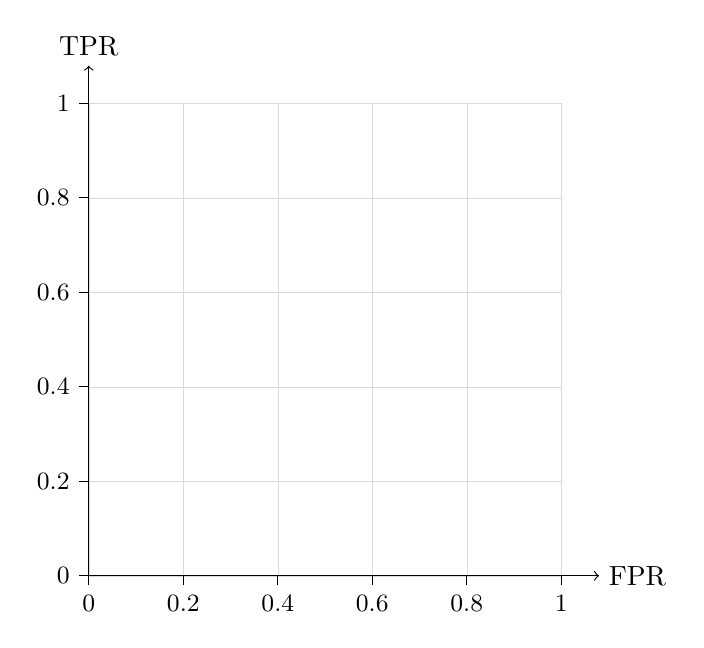
\begin{tikzpicture}[scale=6]\rocaxes\end{tikzpicture}
\end{center}
\fi
\begin{solution}
Sorted by pause, longest first: C (TB), G (TB), F (no), I (TB), A (TB), J (no), D (no), E (TB),
H (no), B (no). As $t$ passes each sample, a TB sample moves the point up by $1/5 = 0.2$ and a
non-TB sample moves it right by $0.2$. Starting at $(0,0)$, the points are
\[
(0,0.2),\ (0,0.4),\ (0.2,0.4),\ (0.2,0.6),\ (0.2,0.8),\ (0.4,0.8),\ (0.6,0.8),\ (0.6,1),\ (0.8,1),\ (1,1).
\]
\begin{center}
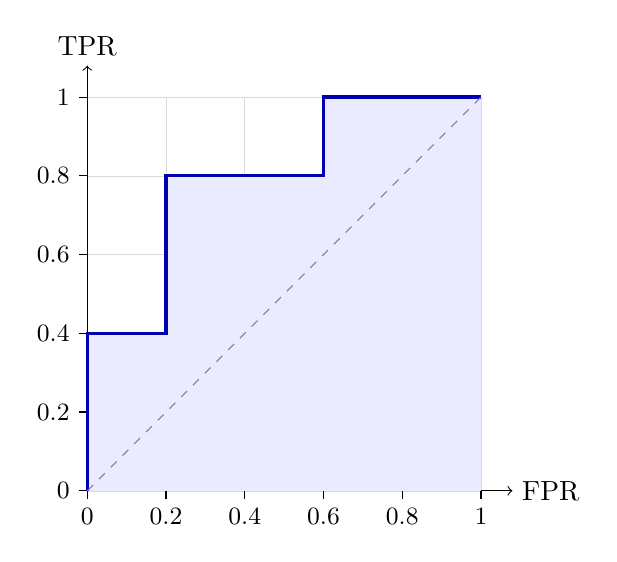
\begin{tikzpicture}[scale=5]
\rocaxes
\fill[blue!8] (0,0) -- (0,0.4) -- (0.2,0.4) -- (0.2,0.8) -- (0.6,0.8) -- (0.6,1) -- (1,1) -- (1,0) -- cycle;
\draw[very thick,blue!70!black] (0,0) -- (0,0.4) -- (0.2,0.4) -- (0.2,0.8) -- (0.6,0.8) -- (0.6,1) -- (1,1);
\draw[dashed,gray] (0,0) -- (1,1);
\end{tikzpicture}
\end{center}
\end{solution}

\part[2] Compute the AUC.
\begin{solution}
The area under the staircase, in columns of width $0.2$ with heights $0.4, 0.8, 0.8, 1, 1$:
$\mathrm{AUC} = 0.2 \times (0.4 + 0.8 + 0.8 + 1 + 1) = 0.80$.
\end{solution}
\end{parts}

% ===================================================================== 2
\titledquestion{Support vector machines (20 points)}
\begin{parts}
\part[10] A soft-margin SVM returned $\bm{w} = (4, 3)$, $b = -12$.
\begin{center}
\begin{tabular}{lccccc}
\toprule
point  & A & B & C & D & E \\
\midrule
$x_1$  & 3 & 1 & 2.5 & 1 & 3 \\
$x_2$  & 1 & 2 & 1 & 2.5 & 0.5 \\
label  & $+$ & $-$ & $+$ & $-$ & $-$ \\
\bottomrule
\end{tabular}
\end{center}
\begin{subparts}
\subpart Compute $f(\bm{x})$ and the predicted class of each point.
\subpart What is the width of the margin?
\subpart Compute each point's distance to the decision boundary.
\subpart Which points are support vectors? Which point is on the margin, which is inside it, and
which is misclassified?
\end{subparts}
\begin{solution}
$f(\bm{x}) = 4x_1 + 3x_2 - 12$ and $\|\bm{w}\| = \sqrt{4^2 + 3^2} = 5$.
\begin{center}
\begin{tabular}{lccccc}
\toprule
point & A & B & C & D & E \\
\midrule
$f(\bm{x})$                     & $3$   & $-2$  & $1$   & $-0.5$ & $1.5$ \\
predicted class                 & $+$   & $-$   & $+$   & $-$    & $+$ \\
distance $|f(\bm{x})|/\|\bm{w}\|$ & $0.6$ & $0.4$ & $0.2$ & $0.1$  & $0.3$ \\
$y\,f(\bm{x})$                  & $3$   & $2$   & $1$   & $0.5$  & $-1.5$ \\
\bottomrule
\end{tabular}
\end{center}
(b) Margin width $= 2/\|\bm{w}\| = 2/5 = 0.4$.

(d) The support vectors are the points with $y\,f(\bm{x}) \le 1$: C, D and E. C is on the margin
($y\,f = 1$), D is inside the margin but correctly classified ($y\,f = 0.5$), and E is
misclassified (label $-$, predicted $+$).
\end{solution}

\part[6] Write down the objective function for the soft-margin SVM and explain why this is what we
want to optimize.
\begin{solution}
\[
\min_{\bm{w},\, b,\, \bm{\xi}} \ \tfrac12 \|\bm{w}\|^2 + C \sum_i \xi_i
\quad \text{subject to} \quad y_i(\bm{w} \cdot \bm{x}_i + b) \ge 1 - \xi_i,\ \ \xi_i \ge 0 .
\]
Minimizing $\tfrac12\|\bm{w}\|^2$ maximizes the margin $2/\|\bm{w}\|$. The slack $\xi_i$ measures
how far point $i$ falls short of being on the correct side, outside the margin; the sum penalizes
these violations. $C$ sets the trade-off between a wide margin and few violations.
\end{solution}

\part[2] Suppose our soft-margin SVM obtains 95\% training accuracy but 60\% validation accuracy.
What does this suggest about our hyperparameter $C$?
\begin{solution}
The large gap between training and validation accuracy means the model overfits. $C$ is probably
too large: violations are so expensive that the margin narrows to fit individual training points.
Try a smaller $C$ (wider margin, more slack), chosen on validation data.
\end{solution}

\part[2] What are support vectors? Is every training datapoint that falls inside the margin a
support vector?
\begin{solution}
Support vectors are the training points that determine the solution: the points on the margin,
inside it, or misclassified, that is, those with $y_i f(\bm{x}_i) \le 1$. Moving any other point
(while it stays outside the margin) does not change the SVM. Yes: every point inside the margin is a
support vector.
\end{solution}
\end{parts}

\end{questions}
\end{document}
